\documentclass{article}
% translate with >> pdflatex -shell-escape <file>

% This file is used as unit test for pgfplots, copyright by Christian Feuersaenger.
% 
% See
%   http://pgfplots.sourceforge.net/pgfplots.pdf
% for pgfplots.
%
% Any required input files (for <plot table> or <plot file> or the table package) can be downloaded
% at
% http://www.ctan.org/tex-archive/graphics/pgf/contrib/pgfplots/doc/latex/
% and
% http://www.ctan.org/tex-archive/graphics/pgf/contrib/pgfplots/doc/latex/plotdata/

\usepackage{pgfplots}
\pgfplotsset{compat=1.3}

\pagestyle{empty}

\begin{document}

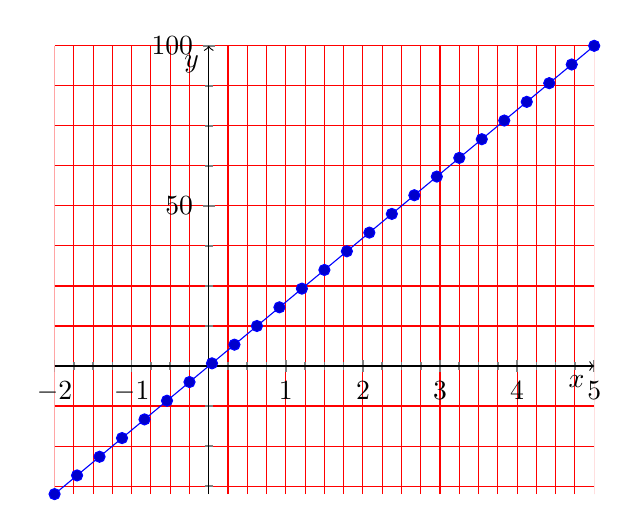
\begin{tikzpicture}
	\begin{axis}[
		axis x line=center,
		axis y line=center,
		 enlargelimits=false,
		grid=both,
		minor tick num=3,
		grid style={draw=red},
		tick style={semithick},
		tick align=center,
		xlabel=$x$,
		ylabel=$y$,
		every axis x label/.style={at={(current axis.right of origin)},anchor=north east},
		every axis y label/.style={at={(current axis.above origin)},anchor=north east},
		axis line style={->},
	]
	\addplot plot[domain=-2:5] (\x,20*\x);
	\end{axis}
\end{tikzpicture}
\end{document}
